\subsection{Modellazione di protocolli con UML}
%\fixnote{mr}{non possiamo avere cos\`i tanti esempi senza spiegazione. O li raccontiamo o li togliamo. Se ``spaccano'' troppo il testo possiamo spostarli in appendice. Inoltre le immagini sono difficili da leggere perch\'e ci sono troppi a-capo nei blocchi. Inoltre le varie immagini sono zoomate diversamente, io renderei pi\`u omogeneo.}
\subsubsection*{Needham Schroeder Symmetric Key}
In questa sezione vedremo come è possibile modellare attraverso i diagrammi object diagram dello standard UML il protocollo di sicurezza a chiave simmetrica proposto da Needham e Schroeder:
\begin{lstlisting}[mathescape]
    1. $A \rightarrow S : A, B, N_a$
    2. $S \rightarrow A : \{N_a, K_{ab}, B, \{K_{ab}, A\}_{K_{bs}}\}_{K_{as}}$
    3. $A \rightarrow B : \{K_{ab}, A\}_{K_{bs}}$
    4. $B \rightarrow A : \{N_b\}_{K_{as}}$
    5. $A \rightarrow B : \{N_b-1\}_{K_{as}}$
\end{lstlisting} 

\noindent Nelle Figure seguenti avremo i seguenti partecipanti al protocollo: l'agente Initiator che vuole iniziare la comunicazione con l'agente Recipient e richiede la password per la comunicazione al server S.\\
Inoltre la chiave simmetrica viene rappresentata in questo modo SK(a,b), dove a e b indicano l'identità degli agenti proprietari della chiave.\\

\begin{figure}[h!] 
    \centering 
    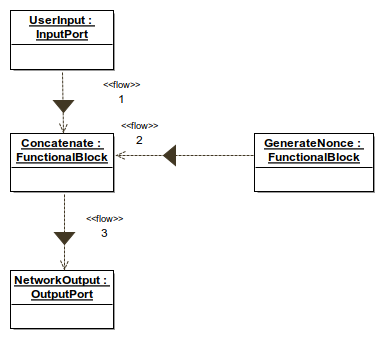
\includegraphics[scale=0.6]{img/NSSK/First_message(toServer)_Object diagram.png} 
    %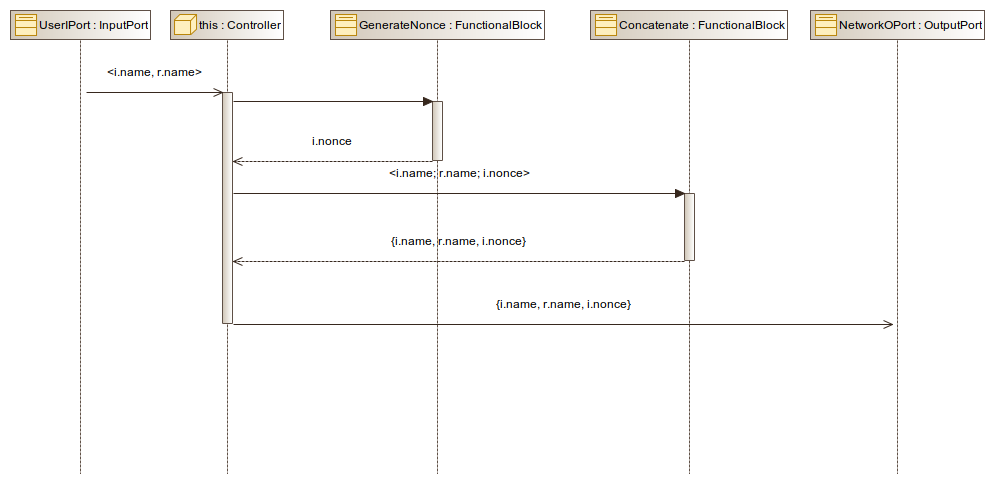
\includegraphics[width=\textwidth]{img/NSSK/Sequencediagram/First_Message(toServer).png} 
    \begin{lstlisting}[frame=single, mathescape, basicstyle=\footnotesize]
        1. $<i.name, r.name>$
        2. $<i.nonce>$
        3. $<i.name, r.name, i.nonce>$
    \end{lstlisting}
    \caption{$A \rightarrow B : A, B, N_a$} 
\end{figure}
\noindent Nell'oggetto UserInput il sistema che andrà ad implementare il protocollo riceve il nome ($r.name$) dell'agente Recipient, l'oggetto GenerateNonce genera un nuovo Nonce e l'oggetto Concatenate prepare il pacchetto, da mandare al server S attaverso l'oggetto NetworkOPort, composto da $i.name, r.name, i.nonce$, ovvero dai nomi dei partecipanti al protocollo e il nonce per assicurarsi che la comunicazione sia fresh.
\newpage
\begin{figure}[h!] 
    \centering 
    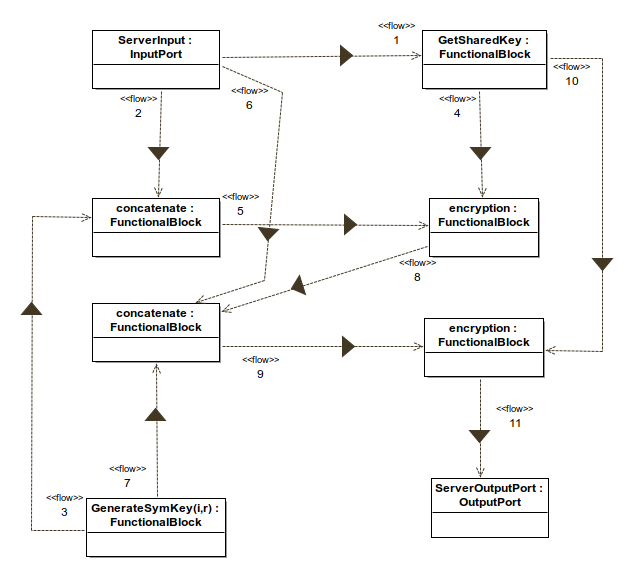
\includegraphics[scale=0.5]{img/NSSK/Second_Message(fromServer).png} 
    %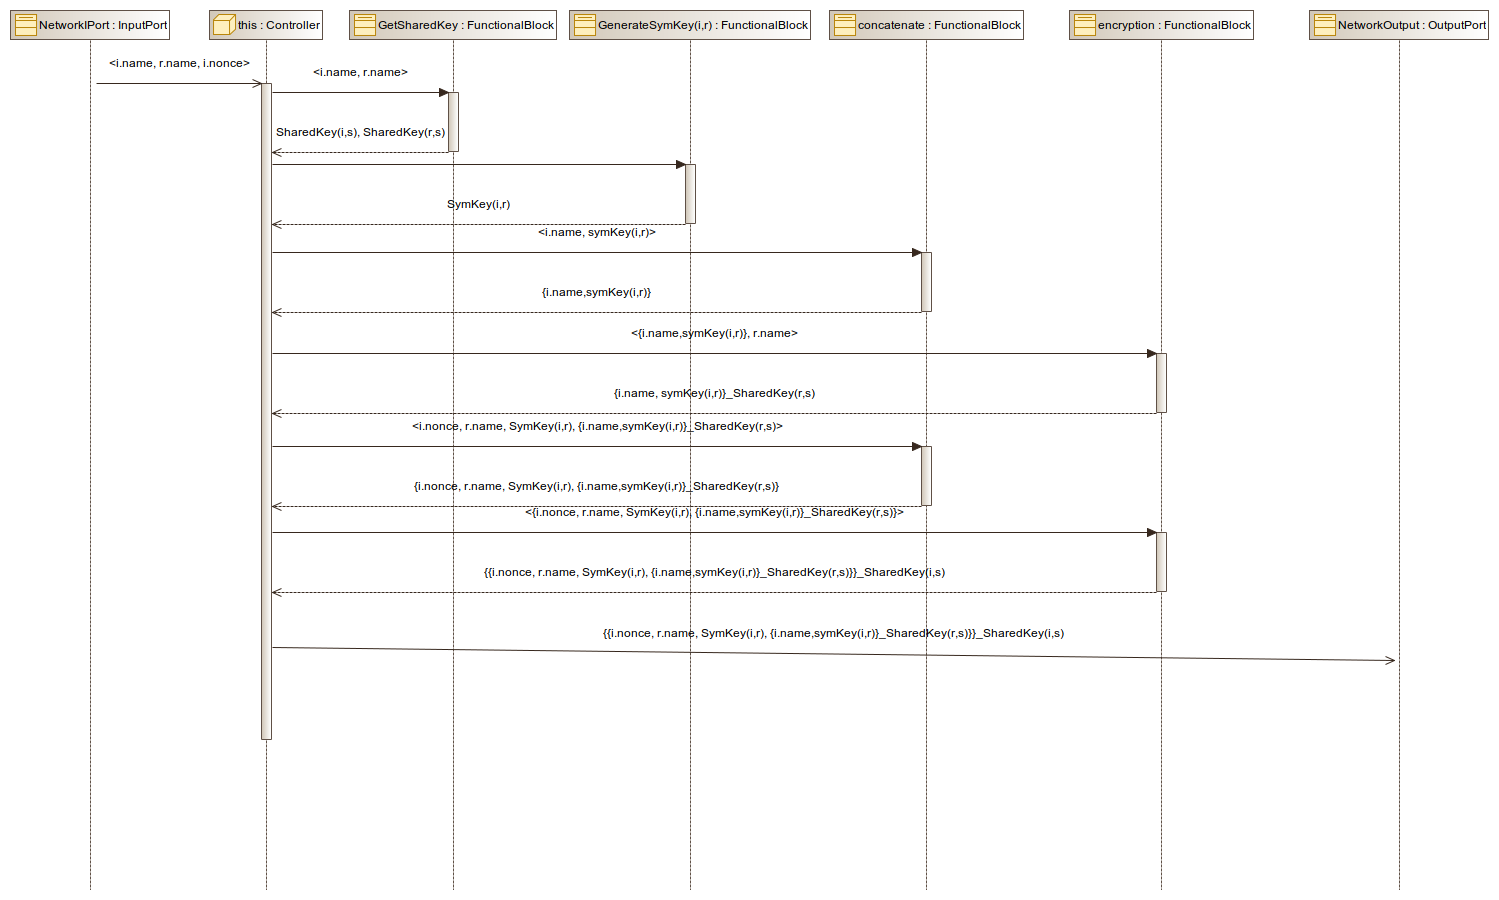
\includegraphics[width=\textwidth]{img/NSSK/Sequencediagram/Second_Message(fromServer).png} 
    \begin{lstlisting}[frame=single, mathescape, basicstyle=\footnotesize]
        1. $<i.name,r.name>$
        2. $<i.name>$
        3. $<SK(i,r)>$
        4. $<SK(s,r)>$
        5. $<i.name, SK(i,r)>$
        6. $<r.name, i.nonce>$
        7. $<SK(i,r)>$
        8. $<\{i.name; SK(i,r)\}\_SK(r,s)>$
        9. $<i.nonce, r.name, SK(i,r), \{i.name,SymKey(i,r)\}\_SK(r,s)\}>$
        10. $<SK(s,r)>$
        11. $<\{i.nonce, r.name, SK(i,r), \{i.name,SK(i,r)\}\_SK(rs)\}\}\_SK(i,s)>$
    \end{lstlisting}
    \caption{$S \rightarrow A : \{N_a, K_{ab}, B, \{K_{ab}, A\}_{K_{bs}}\}_{K_{as}}$} 
\end{figure}
\noindent Una volta ricevuto il pacchetto, il server S provvede alla generazione della chiave simmetrica (SK(i,r)) per la comunicazione tra Initiator e Recipient utilizzando l'oggetto GenerateSymKey(i,r), passando a quest'ultimo i nomi $i.name, r.name$ dei partecipanti.\\ 
A questo punto, fornendo sempre come input i nomi dei partecipanti all'oggetto GetSharedKey, ottiene le chiavi simmetriche precedentemente condivise tra lui e ogni agente partecipante (SK(i,s) e SK(r,s)).\\ 
La chiave SK(r,s) verrà utilizzata dall'oggetto encryption dopo aver preparato con l'oggetto Concatenate il pacchetto per l'agente Recipient, questo pacchetto a sua volta verrà inserito da un altro oggetto Concatenate nel pacchetto per l'agente Initiator e il tutto verrà cifrato da un'altro oggetto encryption con la chiave SK(i,s). Il pacchetto risultante da queste operazioni verrà spedito all'agente Initiator attraverso l'oggetto ServerOutputPort.\\

\begin{figure}[h!] 
    \centering 
    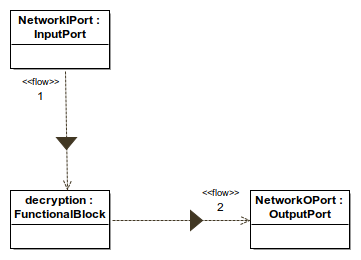
\includegraphics[scale=0.6]{img/NSSK/FirstMessage.png} 
    %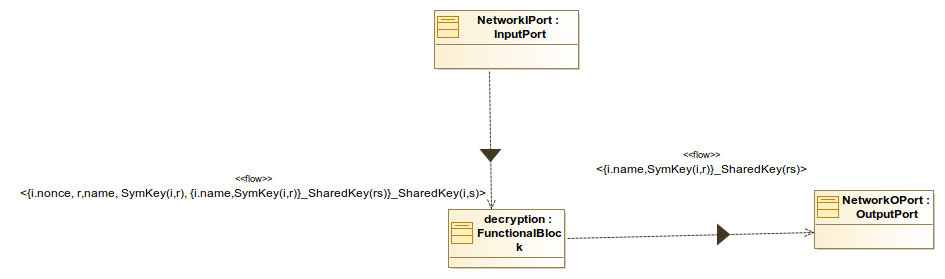
\includegraphics[width=\textwidth]{img/NSSK/Sequencediagram/FirstMessage.png}
    \begin{lstlisting}[frame=single, mathescape, basicstyle=\footnotesize]
        1. $<\{i.nonce, r.name, SK(i,r), \{i.name,SK(i,r)\}\_SK(r,s)\}\_SK(i,s)>$
        2. $<\{i.name,SK(i,r)\}\_SK(r,s)>$
    \end{lstlisting}
    \caption{$A \rightarrow B : \{K_{ab}, A\}_{K_{bs}}$} 
\end{figure}
\noindent L'agente Initiator riceve il pacchetto attraverso l'oggetto NetworkIPort e utilizza l'oggetto di decryption con la chiave simmetrica SK(i,s) per estrarre il pacchetto da inoltrare all'agente Recipient attraverso l'oggetto NetworkOPort.\\
\begin{figure}[h!] 
    \centering 
    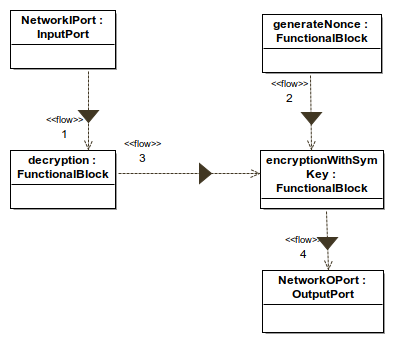
\includegraphics[scale=0.59]{img/NSSK/SecondMessage.png} 
    %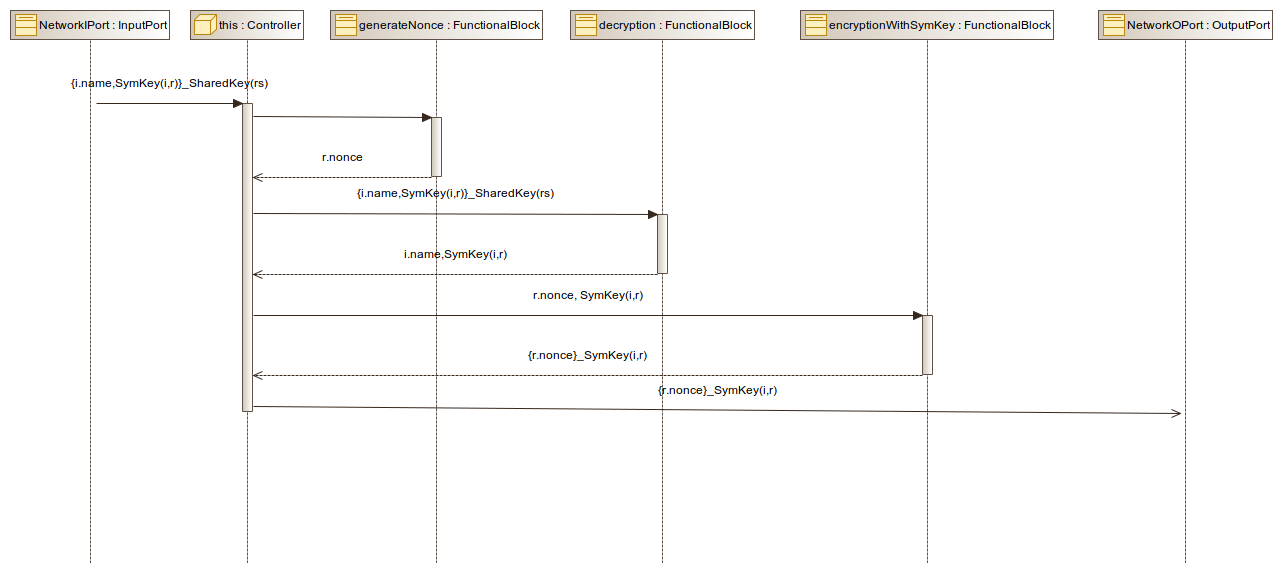
\includegraphics[width=\textwidth]{img/NSSK/Sequencediagram/SecondMessage.png} 
    \begin{lstlisting}[frame=single, mathescape, basicstyle=\footnotesize]
        1. $<\{i.name,SK(i,r)\}\_SK(r,s)>$
        2. $<r.nonce>$
        3. $<SK(i,s)>$
        4. $<\{r.nonce\}\_SK(i,r)>$
    \end{lstlisting}
    \caption{$B \rightarrow A : \{N_b\}_{K_{as}}$} 
\end{figure}
\newpage
\noindent L'agente Recipient riceve il pacchetto attraverso l'oggetto NetworkIPort, lo decifra con l'oggetto decryption utilizzando la chiave SK(r,s) ed estrae la chiave SK(i,r).\\ 
SK(i,r) verrà utilizzata dall'oggetto encryptionWithSymKey per cifrare un nuovo pacchetto contenente il Nonce generato dall'oggetto generateNonce.\\ 
Infine l'agente Recipient spedisce il pacchetto all'agente Initiator utilizzando l'oggetto NetworkOPort.\\
\begin{figure}[h!] 
    \centering 
    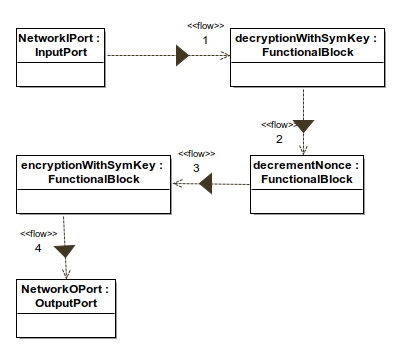
\includegraphics[scale=0.6]{img/NSSK/ThirdMessage.png} 
    %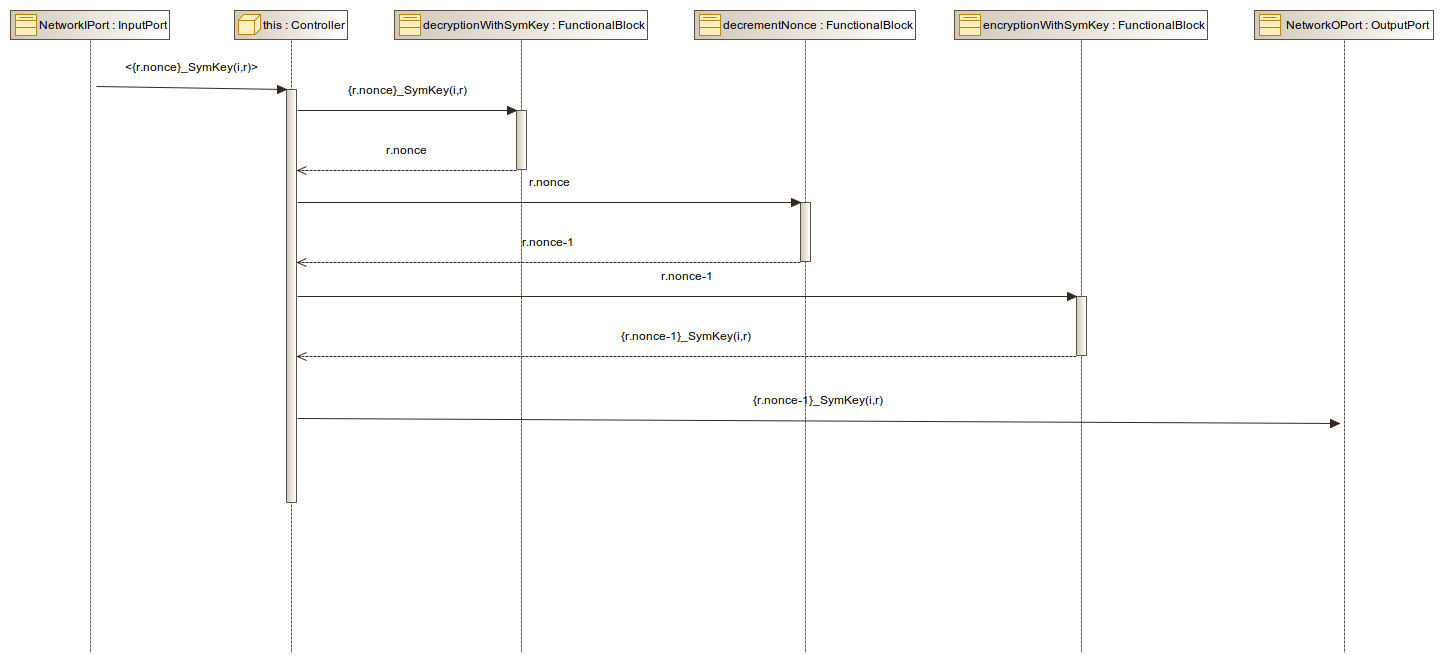
\includegraphics[width=\textwidth]{img/NSSK/Sequencediagram/ThirdMessage.png} 
    \begin{lstlisting}[frame=single, mathescape, basicstyle=\footnotesize]
        1. $<{r.nonce}\_SK(i,r)>$
        2. $<r.nonce>$
        3. $<r.nonce-1>$
        4. $<\{r.nonce-1\}\_SK(i,r)>$
    \end{lstlisting}
    \caption{$A \rightarrow B : \{N_b-1\}_{K_{as}}$} 
\end{figure}\\
\noindent Nell'ultima fase del protocollo, l'agente Initiator riceve dall'oggetto NetworkIPort il pacchetto contenente il Nonce, lo decifra con l'oggetto decryptionWithSymKey utilizzando la chiave SK(i,r), utilizza l'oggetto decrementNonce per sottrarre 1 al Nonce inviato dall'agente Recipient e cifra il risultato con l'oggetto encryptionWithSymKey utilizzando la chiave SK(i,r).\\
Il pacchetto risultante viene spedito all'agente Recipient attraverso l'oggetto NetworkOPort.\\

\newpage
\subsubsection*{Address Resolution Protocol}
Lo scopo del protocollo ARP descritto in \cite{RFC0826} e in \cite{RFC5227} è quello di eseguire una mappatura tra indirizzo IP e indirizzo MAC di una macchina all'interno di una rete locale Ethernet.\\
La notazione seguente utilizzata nei pacchetti è ripresa da \cite{RFC0826}:
\begin{lstlisting}
    ar$hrd: Hardware address space 
    ar$pro: Protocol address space
    ar$hln: byte length of each hardware address
    ar$pln: byte length of each protocol address
    ar$op:  opcode (request | reply)
    ar$sha: Hardware address of sender 
    ar$spa: Protocol address of sender 
    ar$tha: Hardware address of target
    ar$tpa: Protocol address of target
\end{lstlisting}
In Figura \ref*{fig:ARP} vediamo come si modella il protocollo ARP.\\
Una macchina, appena connessa alla rete o accesa, si mette subito in ascolto con l'oggetto ANNUNCE\_AWAIT e, allo stesso tempo, utilizza gli oggetti getIPAddress per generare un indirizzo IP sul quale essere contattata, getProtocolType e getMACAddress  per ricavare informazioni sul tipo di protocollo ethernet da utilizzare e l'indirizzo MAC della sua scheda di rete.\\
A questo punto utilizza queste informazioni per creare attraverso l'oggetto createProbePackage un pacchetto da inviare in broadcast a tutte le macchine della rete.\\
Successivamente attende un tempo predefinito attraverso l'oggetto PROBE\_WAIT, prima di spedire il pacchetto attraverso l'oggetto EthernetOUT e ritornare nello stato di ANNUNCE\_WAIT.\\
Se nell'arco di un tempo predefinito non arriva nessun pacchetto dall'oggetto EthernetIN, procede con la conferma dell'indirizzo IP attraverso la creazione di un nuovo pacchetto con l'oggetto createAnnuncePackage, il quale verra sempre spedito in broadcast attraverso l'oggetto EthernetOUT.\\
Se invece riceve un pacchetto dall'oggetto EthernetIN, ricomincia generando un nuovo indirizzo IP.\\
\newpage
\begin{figure}[h!] 
    \centering 
    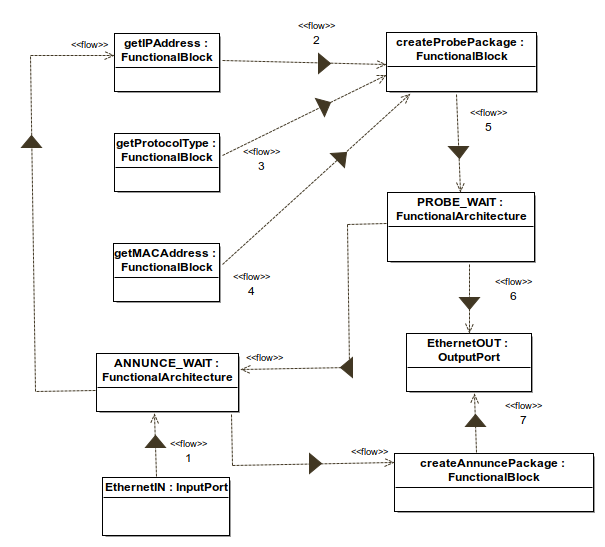
\includegraphics[scale=0.6]{img/ARP/ARP.png} 
    \begin{lstlisting}[frame=single, mathescape, basicstyle=\footnotesize]
1. $<\{as\$hrd, ar\$pro, ar\$hln, ar\$pln, reply, ar\$sha, ar\$spa, ar\$tha, ar\$tpa\}>$
2. $<ip>$
3. $<ar\$spa>$
4. $<ar\$sha>$
5. $<\{as\$hrd, ar\$pro, ar\$hln, ar\$pln, request, ar\$sha, 0.0.0.0, 00:00:00:00:00:00, ip\}>$
6. $<\{as\$hrd, ar\$pro, ar\$hln, ar\$pln, request, ar\$sha, 0.0.0.0, 00:00:00:00:00:00, ip\}>$
7. $<\{as\$hrd, ar\$pro, ar\$hln, ar\$pln, request, ar\$sha, ip, 00:00:00:00:00:00, ip\}>$
    \end{lstlisting}
    \caption{Modellazione del protocollo ARP} 
    \label{fig:ARP}
\end{figure}
\newpage
\begin{figure}[h!] 
    \centering 
    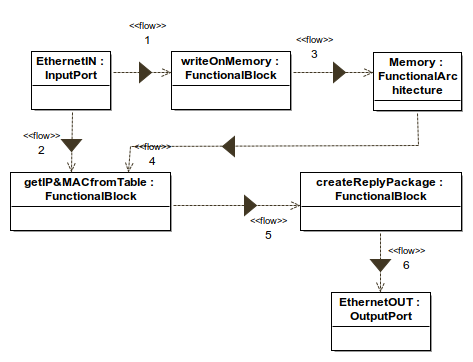
\includegraphics[scale=0.6]{img/ARP/ARP_Reply_Object_diagram.png} 
\begin{lstlisting}[frame=single, mathescape, basicstyle=\footnotesize]
1. $<\{as\$hrd, ar\$pro, ar\$hln, ar\$pln, request, ar\$sha, ip, 00:00:00:00:00:00, ip\}>$
2. $<\{as\$hrd, ar\$pro, ar\$hln, ar\$pln, request, ar\$sha, 0.0.0.0, 00:00:00:00:00:00, ip\}>$
3. $<ar\$sha, ip>$
4. $<ar\$tha, ar\$tpa>$
5. $<ar\$tha, ar\$tpa>$
6. $<\{as\$hrd, ar\$pro, ar\$hln, ar\$pln, reply, ar\$sha, ar\$spa, ar\$tha, ar\$tpa\}>$
\end{lstlisting}
    \caption{Modellazione del blocco di ARP Reply} 
\end{figure}
\noindent Nel caso in cui una macchina della rete riceva un pacchetto dall'oggetto EthernetIN, la prima cosa che fa è verificare se si tratta di un pacchetto di probe oppure di un pacchetto di annunce.\\
Nel primo caso va a verificare con l'oggetto Memory se nell'ARP cache è già presente quell'indirizzo IP, assegnato ad un indirizzo MAC, che non corrisponde a quello del sender del pacchetto.\\ 
Se vi è una corrispondenza tra l'indirizzo ip del sender del pacchetto ed uno già presente nell'ARP cache, allora l'oggetto getIP\&MACFromTable riceve in input le informazioni dalla ARP cache per generare un nuovo pacchetto attraverso l'oggetto createReplyPackage, con il quale rispondere in unicast al sender attraverso l'oggetto EthernetOut, altrimenti non fa nulla.\\
Nel caso in cui si tratti di un pacchetto di annunce allora l'oggetto writeOnMemory si occuperà di salvare nella ARP cache la mappatura tra l'indirizzo IP e MAC del sender.\\
\newpage
\clearpage
\subsubsection*{RSA}
Nel 1978 in \cite{RSA78} Rivest, Shamir e Adleman hanno proposto un crittosistema per la cifratura e la firma dei messaggi basato sulla crittografia asimmetrica.\\
Come vedremo nelle Figure successive il crittosistema si basa su tre funzioni principali: funzione di generazione delle chiavi, funzione di encryption e funzione di decryption.\\
Nella modellazione UML ogni oggetto rappresenta le funzioni matematiche utilizzate dalle tre funzioni.\\ 
L'oggetto Memory viene utilizzato dalla funzione di generazione delle chiavi per salvare le informazioni riguardo la chiave pubblica e la chiave privata necessarie alle funzioni di encryption e decryption.\\  
\begin{figure}[h!] 
    \centering 
    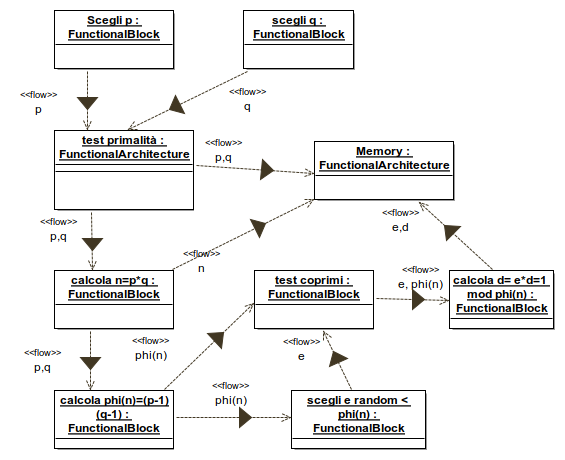
\includegraphics[scale=0.6]{img/RSA/Key_Generation_Object_diagram.png} 
    \caption{Generazione delle chiavi} 
\end{figure}
\begin{figure}[h!] 
    \centering 
    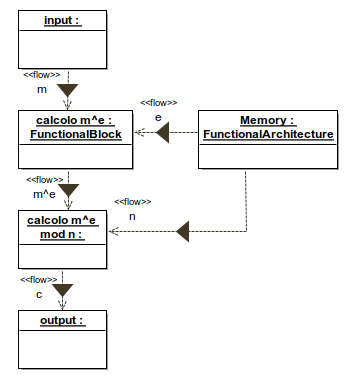
\includegraphics[scale=0.6]{img/RSA/Encryption_Object_diagram.png} 
    \caption{Funzione di encryption} 
\end{figure}
\newpage
\begin{figure}[h!] 
    \centering 
    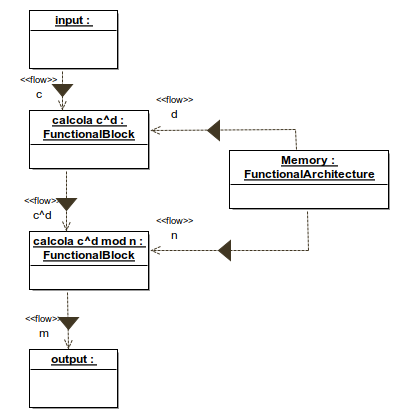
\includegraphics[scale=0.6]{img/RSA/Decryption_Object_diagram.png} 
    \caption{Funzione di decryption} 
\end{figure}
\newpage



    
